
\subsubsection{Test Run Data Acquisition}
\label{sec:testrun_daq}
%This section describes the overall design of the DAQ system used in the test run. 
%Considering the similarity to the 
%system proposed for HPS only a brief description is given here, with an emphasis on the differences. 
%Results, milestones and experiences attained from operating the DAQ in the test run is also presented. 

%The DAQ system for the HPS test run handles the data and trigger distribution for the ECal and SVT. 

The data acquisition system for the HPS test run was a somewhat simplified version of the DAQ proposed for the
full experiment, described in Sec.~\ref{sec:daq}, and proves the principles of the design.  In addition to simpler trigger logic,
the primary differences for the ECal are a different data path and simplified trigger logic that results in somewhat worse
single-crystal energy resolution and precludes calibration of individual crystal gains at the trigger level.  For the SVT, the smaller
number of channels eliminated the need for optical conversion and aggregation of data and detector power inside the vacuum chamber.
Finally, most data links had 1 Gbit/s bandwidth, sufficient for the purposes of the test run.

In other respects, the Test Run DAQ is essentially identical to that proposed for HPS.  The ECal provides data to the FADC-based Level~1
trigger system. Accepted events are read out from the ECal and SVT DAQ and processed by an event builder before output to disk.
For the ECal, the Readout Crate Controllers (ROCs) are the same as those proposed for HPS and are installed in VME, VME64X and VXS 
crates running mvme6100 controllers, with prpmc880 or pmc280 co-processor modules. For simplicity, a hybrid approach was 
used for the SVT DAQ in the test run where the ROC ran on a external PC connected to the ATCA crate. As proposed for HPS, a 
Foundry Router was used as the backbone of the DAQ system, providing 1~Gbit/s and 10~Gbit/s connections between components 
and to the JLAB Computer Center. The Event Builder, Event Recorder, and other critical DAQ components ran on 4-CPU Opteron-based servers, 
which was sufficient for the test run. The RAID5 storage system had 100~MB/s capability to handle the anticipated data rates for electron running.


%The DAQ system built for the HPS test run was a proof of principle for that proposed for HPS, described in 
%Sec.~\ref{sec:daq}. Consequently, the architecture of the systems are very similar. The main differences 
%for the ECal and trigger, in addition to the simpler trigger logic, is a different trigger and readout data 
%path. This resulted in a lower crystal energy resolution and no possibility of crystal gain calibration at the 
%trigger level. The smaller SVT relaxed the need for optical conversion and for signal and power aggregation 
%inside the vacuum chamber. 
%Most of the data links were 1~Gbit/s bandwidth, large enough given the data rates expected in the test run.
%
%
%
%The two front-end electronics systems for the ECal and SVT are essentially unchanged compared to the HPS 
%DAQ system. The ECal provides 
%input to the Level~1 trigger system after which an accepted event is acquired from the two sub-systems 
%and are processed. The Readout Crate Controllers (ROCs)
% described for HPS are unchanged and installed in every VME, VME64X, VXS crates running 
% mvme6100 controllers with a prpmc880 or pmc280 co-processor modules. A hybrid approach was 
% used for the SVT DAQ in the test run where the ROC ran on a external PC connected to the ATCA crate. 
% Similar to HPS, a Foundry Router was used as the backbone of the DAQ system, providing 1~Gbit/s and 
% 10~Gbit/s connections between components and to the JLAB Computer Center. The Event Builder, Event 
% Recorder, and other critical DAQ components ran on 4-CPU Opteron-based servers, which was sufficient 
% for the test run. The RAID5 test run storage system had a 100~MB/s capability to handle the data rates 
% expected for the test run as described below.

%\subsubsection{SVT DAQ}

The SVT DAQ was designed to read out data continuously at 40~MHz from the SVT modules and transfer data 
to the JLab DAQ once a trigger signal is received. It is based on the same overall architecture as the system 
described in Sec.~\ref{sec:svt_daq}. Being only half the size of the HPS SVT, the largest difference is the provision for
individual power and data for each sensor and readout chip from the power supplies and DAQ outside of the vacuum chamber.
This simplification reduced development time and cost at the expense of a large number of connections and vacuum feedthroughs.
With a total of 20 silicon microstrip sensors, each one connected to an onboard hybrid readout 
card hosting five 128-channel APV25 ASICs (shown in Figure ~\ref{fig:hybrid_and_apv25_testrun}), 600 lines for power and data are required.
 \begin{figure*}[t]
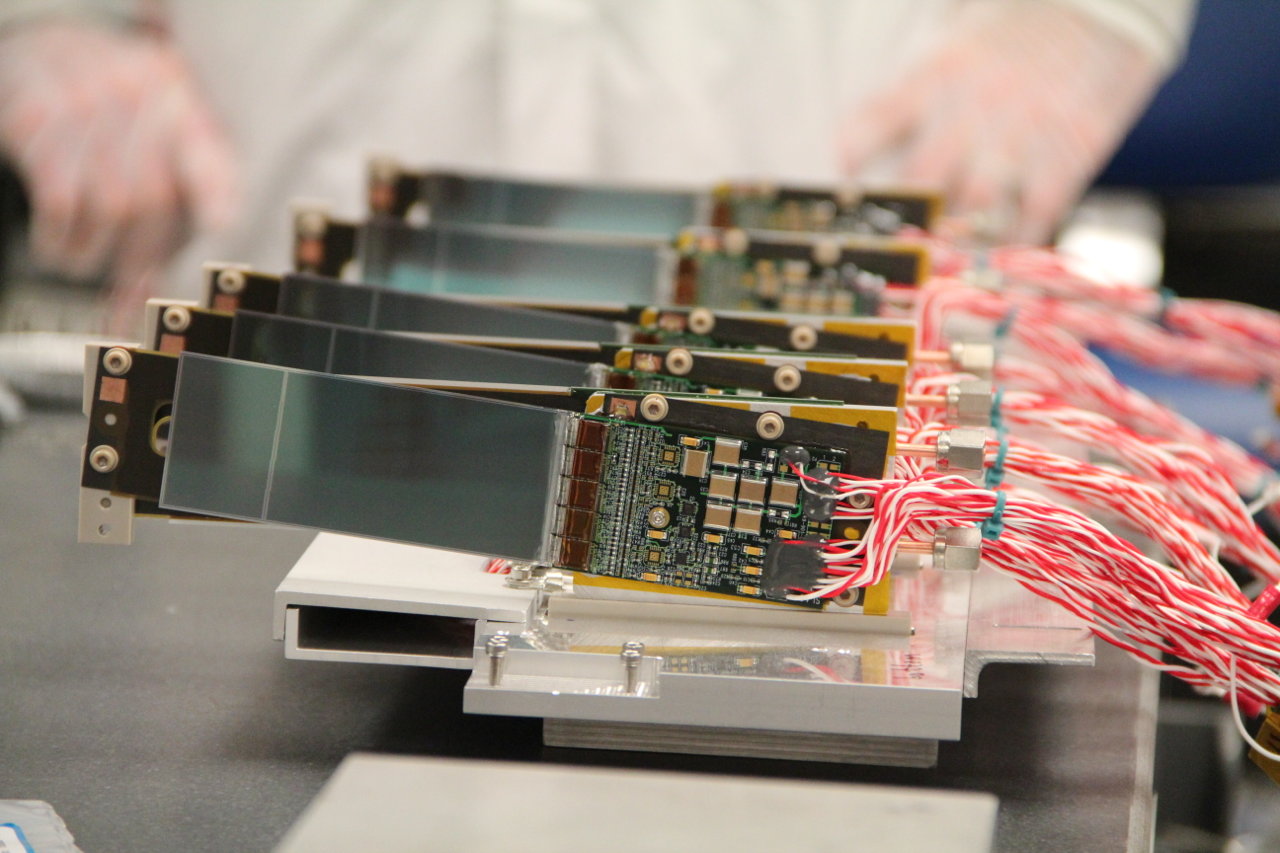
\includegraphics[ scale=0.3]{test2012/daq/svt_modules_on_sup_plate.png}
\caption{\small{View from upstream of one half of the SVT modules mounted on the support plate. Signal, 
power and control are soldered, and potted, to pads at one end while the five APV25 chips are wirebonded 
to the silicon sensor at the other.}}
\label{fig:hybrid_and_apv25_testrun}
\end{figure*}
Without optical conversion inside the chamber as proposed for HPS, analog signals from the APV25 chips are 
carried directly to the ATCA crate located outside the vacuum chamber via multi-twisted-pair cable. 
The amplification and digitization is carried out on a Rear Transition Module (RTM) board designed specifically for the HPS test run. 
On the RTM, a pre-amplifier converts the APV25 differential current output to a voltage output 
scaled to the sensitive range of a 14-bit ADC. The RTM is organized into four sections with each section 
supporting 3 hybrids (15 channels). The ADC is operated at the system clock of 41.667~MHz. 
%The RTM also includes a 4-channel Fiber Optic module and supporting logic which can be used to interface to the JLAB trigger supervisor card.
The ATCA main board, the Cluster on Board (COB), is similar to the one described for the HPS DAQ 
with the important exception that one of the Data Processing Modules (DPMs) functions as the trigger 
interface and there is no Reconfigurable Cluster Element (RCE) module. Instead, the DPMs that package and send the data from the hybrids to 
an external PC through a 1~Gbit/s ethernet connection serve the same purpose as the 
RCE module in the HPS DAQ. Figure~\ref{fig:svtdaq} shows an overall layout of 
the SVT DAQ system used for the test run (compare to Fig.~\ref{fig:svt_daq_overview}).
 \begin{figure}[t]
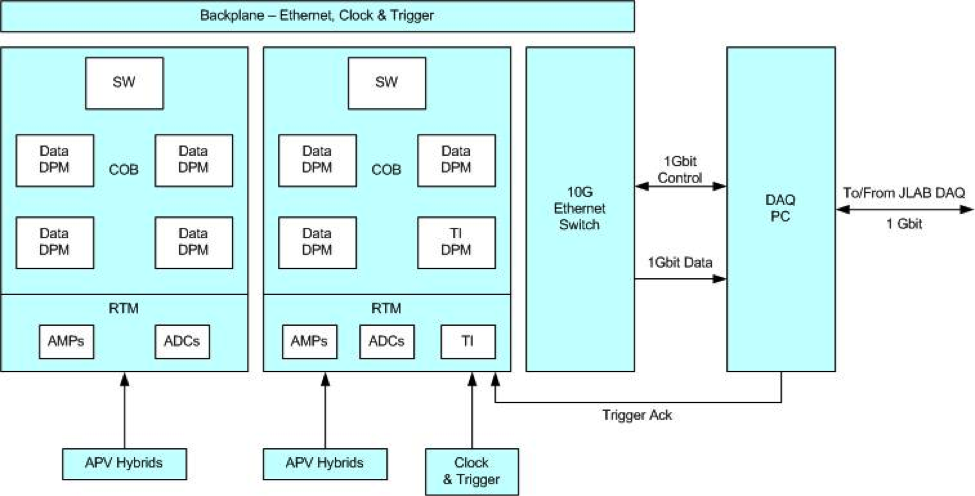
\includegraphics[scale=0.9]{test2012/daq/svt_daq_diagram.png}
\caption{\small{Schematic of the SVT DAQ used for the test run. Note that the hybrids are connected directly 
to the RTM and that an external DAQ PC is used for control and transfer of data to the JLab DAQ.}}
\label{fig:svtdaq}
\end{figure}
The ATCA crate hosts two COB cards, one supporting four data processing DPMs and the other supporting three data processing DPMs and one trigger DPM for a capacity of 21 hybrids, one more than required. 
The test run RTM and COB boards are shown in Fig.~\ref{fig:rtm_testrun}. 
\begin{figure*}[t]
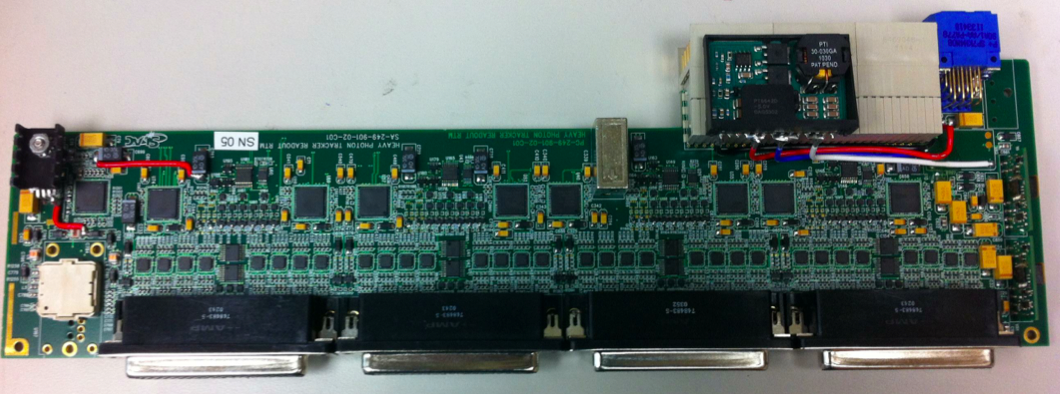
\includegraphics[ scale=0.25]{test2012/daq/rtm.png}
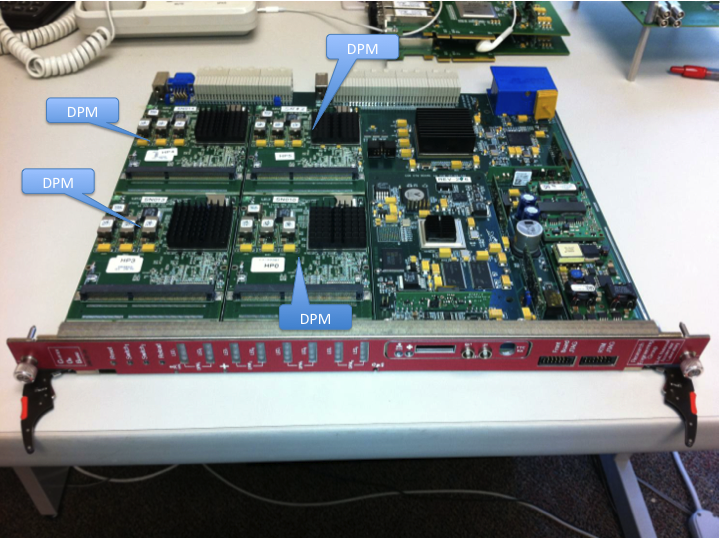
\includegraphics[ scale=0.4]{test2012/daq/svt_daq_module_noted.png}
\caption{\small{Picture of a RTM (top) and COB board (bottom) used in the HPS test run 2012.}}
\label{fig:rtm_testrun}
\end{figure*}
The external PC supports three network interfaces, two standard 1~Gbit/s Ethernet and one custom low latency 
data reception card. The first Ethernet interface is used for slow control and monitoring of the eight 
DPM modules. The second Ethernet interface serves as the interface to the JLAB data acquisition system. The
low latency network interface is used to receive data from the SVT ATCA crate and supports a low latency, 
reliable, TTL trigger acknowledge interface to the trigger DPM. This PC hosts the SVT control and monitoring 
software as well as the ROC application described above.



Signals from each module are sent to a signal splitter. One of the outputs of the splitter is fed to a discriminator that also has an internal scaler, and then to a TDC channel. The other output is sent to the Jefferson Lab FADC250 VXS module, Figure \ref{fig:fadc}. Two FADC crates are required for the  two modules. The trigger from the ECal is based on FADC information and includes a cluster finding algorithm using FPGA modules. It is described in Section \ref{trigger}. With the FADCs, the energy of clusters will be determined at the crate trigger level and will be used in making the trigger decision.

\begin{figure}[t]
\includegraphics[scale=0.5]{test2012/daq/FADC250_Photo_001.jpg}
\caption{\small{FADC250 VXS module.}}\label{fig:fadc}
\end{figure}




